% arara: pdflatex: { shell: yes, interaction: nonstopmode }
% arara: pythontex: {verbose: yes, rerun: modified }
% arara: pdflatex: { shell: yes, interaction: nonstopmode }
% arara: clean: { extensions: [ aux, blg, idx, ilg, ind, log, out, pytxcode, rel, toc ] }
% !arara: clean: { files: [ ans.tex, hint.tex] }

% arara: pdflatex
% arara: clean: { extensions: [ aux, blg, idx, ilg, ind, log, out, pytxcode, rel, toc ] }
% !arara: clean: { files: [ ans.tex, hint.tex] }


\documentclass[queueing-book-solution.tex]{subfiles}
%\externaldocument{queueing-book}

\opt{solutionfiles,check}{
\loadgeometry{tufte}
\Opensolutionfile{hint}
\Opensolutionfile{ans}
}

\begin{document}


\section{$M^X/M/1$ Queue: Expected Waiting Time}
\label{sec:mxm1-queue:-expected}

Sometimes jobs arrive in batches, rather than as single units.
For instance, when a car or a bus arrives at a fast-food restaurant, a batch consists of the number of people in the vehicle.
When the batches arrive as a Poisson process and the individual items within a batch have exponential service times we denote such queueing systems by the shorthand $M^X/M/1$.
For this queueing model we derive expressions for the load,  the expected waiting time and number of jobs in the system.

We will use the renewal-reward theorem in two ways. In the first we focus on entire batches at the server, in the other on single items.


\newthought{Assume that jobs} arrive as a Poisson process with rate $\lambda$ and each \emph{job} contains multiple \emph{items}.
%Let $A_k$ be the arrival time of job $k$ and $A(t)$ the number of (job) arrivals up to time $t$.
Denote by $B_k$ the batch size of the $k$th job.
We assume that $\{B_k\}$ is a sequence of iid discrete rvs that are distributed as a common rv~$B$. The service times of the items in the batch are also iid with common rv~$S$. The utilization is therefore
%\begin{equation*}
$\rho = \lambda \E B \E S$;
%\end{equation*}
As always we require that $\rho<1$.


\newthought{Suppose that an} arriving batch joins the end of the queue (if present), and once the queue in front of it has been cleared, it moves in its entirety to the server.\sidenote{This is the same batching model as in~\cref{sec:setups-batch-proc}.}
Thus, all items in one batch spend the same time in queue.
Once the batch moves to the server, the server processes the items one after another until the batch is finished.
Write $\Q^B$ for the number of batches in queue and $\Ls^B$ for the number of items (if any) at the server.


Observe that the average time $\E{\W^{B}}$ a batch spends in queue is\sidenote{First  the items at the server have to be served, then the ones in queue.}
\begin{align*}
  \E{\W^B} &=  \E{\Ls^B}\E S + \E{\Q^B} \E B \E S.
\end{align*}
But since $\E L = \E{\Ls^B} + \E{\Q^B} \E B$,
\begin{align*}
  \E{\W^B} &=  \E\L \E S = \E{\W},
\end{align*}
where $\E W$ is the average time an \emph{item} spends in queue.
Using this, and replacing in the above $\E{\Q^B}$ by\sidenote{Little's law} $\lambda \E{\W^B}$, we obtain
\begin{align}\label{eq:96}
\E W =  \E{\W^B} &= \frac{\E{\Ls^B}}{1-\rho}\E{S}.
\end{align}
So let us find an expression for $\E{\Ls^B}$.

\newthought{For this we} can use the renewal reward theorem.
With~\cref{eq:little:2} as inspiration, define $Y(t) = \int_0^t \Ls^B(s) \d s$ as the time spent by the items at the server.
By taking $D_k$ as the departure time of the $k$th batch, $X_k = Y(D_k)-Y(D_{k-1})$ then becomes the time spent by the items of the $k$th batch at the server.
A bit of work shows then that\sidenote{\cref{ex:99}}
\begin{equation}\label{eq:9}
  \E X = \frac{\E{B^2}+\E B}2 \E S.
\end{equation}
Since $Y=\lim_{t\to\infty} Y(t)/t = \E{\Ls^{B}}$,
\begin{align}
  \E{\Ls^B} &= \lambda \frac{\E{B^2}}2\E S + \frac\rho 2 \label{eq:17}\\
  &= \frac{1+C_s^2}2 \rho \E B + \frac{\rho}{2},\label{eq:mxm1:1}
\end{align}
where the first equality  follows\sidenote{\cref{ex:100}} from $Y=\lambda X$ and the second after some polishing\sidenote{\cref{q:batch}} and defining $C_s^2 = \V B/ (\E B)^{2}$ as the SCV of the batch size distribution. Finally, substituting this into~\cref{eq:96} gives
\begin{equation}\label{eq:43}
\E{\W} =
\frac{1+C_s^2}2 \frac{\rho}{1-\rho} \E B \E S + \frac12\frac\rho{1-\rho} \E S.
\end{equation}


\newthought{Rather than using} the time an entire batch spends at the server, as in the above use of the renewal-reward equation, we can also concentrate on the time spent by single items at the server.
This will provide us with a simple expression for $\P{\Ls=i}$, which in turn leads to another derivation of~\cref{eq:17}.

If $\Ls(t)$ is the number of items (of the batch in service) at the server at time $t$, then $Y_i(t) = \int_0^t \1{\Ls(s)=i} \d s$ is the total time there are~$i$ items at the server. It follows\sidenote{\cref{fig:remainingservicetime}}
%\begin{equation*}
$\int_{ D_{k-1}}^{D_k} \1{\Ls(s)=i} \d s = \1{B_k \geq i} S_{k,i}$,
%\end{equation*}
where $S_{k,i}$ is the service time of the $i$th item of this batch. But then,
$Y_i(D_n) = \sum_{k=1}^n \1{B_k\geq i} S_{k,i}$.


\begin{figure}[th]
 \centering
 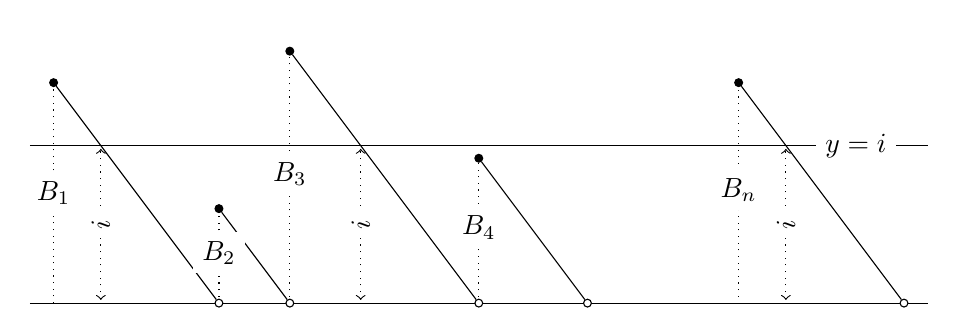
\begin{tikzpicture}[yscale=0.8,xscale=0.6,
 open/.style={shape=circle, fill=white, inner sep=1pt, draw, node contents=},
 closed/.style={shape=circle, fill=black, inner sep=1pt, draw, node contents=}]

 % y = zero line
 \draw (-0.5, 0) -- (18.5, 0);
 % level crossing
 \draw (-0.5, 2.5) -- (18.5, 2.5)
 %node[pos=0.65, fill=white, above] {$\sum_{k=1}^n \1{B_k \geq i}$}
 node[pos=0.92, fill=white] {$y=i$};


 \draw node (c1) at (0,3.5) [closed, label={}]
 node (c2) at (3.5,0)[open, label={}]
 (c1) to (c2);
 \draw[dotted] (0,0) -- (0,3.5) node[midway, fill=white] {$B_1$};
 \draw[dotted, <->] (1, 0.05) -- (1, 2.45) node[fill=white, midway, rotate=90] {$i$};


 \draw node (c1) at (3.5,1.5) [closed, label={}]
 node (c2) at (5,0)[open, label={}]
 (c1) to (c2);
 \draw[dotted] (3.5,0.1) -- (3.5,1.5) node[midway, fill=white] {$B_2$};

 \draw node (c1) at (5,4) [closed, label={}]
 node (c2) at (9,0)[open, label={}]
 (c1) to (c2);
 \draw[dotted] (5,0.1) -- (5,4) node[midway, fill=white] {$B_3$};
 \draw[dotted, <->] (6.5, 0.05) -- (6.5, 2.45) node[fill=white, midway, rotate=90] {$i$};

 \draw node (c1) at (9,2.3) [closed, label={}]
 node (c2) at (11.3,0)[open, label={}]
 (c1) to (c2);
 \draw[dotted] (9,0.1) -- (9,2.3) node[midway, fill=white] {$B_4$};

 % end
 \draw node (c1) at (14.5,3.5) [closed, label={}]
 node (c2) at (18,0)[open, label={}]
 (c1) to (c2);
 \draw[dotted] (14.5,0.1) -- (14.5,3.5) node[midway, fill=white ] {$B_n$};
 \draw[dotted, <->] (15.5, 0.05) -- (15.5, 2.45) node[fill=white, midway, rotate=90] {$i$};


 % bottom line
 %\draw[<->] (0, -0.6) -- (18, -.6) node[fill=white, midway] {$\sum_{k=1}^n B_k$};
\end{tikzpicture}

\caption{A batch crosses the line $y=i$ iff it contains at least $i$ items.
 Thus, during the service of a batch with $i$ or more items, there is precisely one service of an $i$-th item.}
 \label{fig:remainingservicetime}
\end{figure}


By sampling $Y(\cdot)$ at departure times $\{D_k\}$, we see that  $X_k = Y_i(D_k) - Y_i(D_{k-1}) = S_{k,i} \1{B_{k} \geq i}$.
Since the $\{S_{k, i}\}$ are iid\ with $\E{S_{k,i}} = \E S$,
 and the $\{B_k\}$ are iid, we obtain
 \begin{equation*}
X = \lim_{n\to\infty} \frac{1}{n}\sum_{k=1}^n S_{k,i} \1{B_{k} \geq i} = \E{S \1{B\geq i}}.
 \end{equation*}
 But $B$ and $S$ are independent by assumption, hence $X = \E{S} \E{\1{B\geq i}} = \E S G(i-1)$, since $G$ is the survivor function of $B$.
 As for $Y$, by construction, $Y_i(t)/t \to \P{\Ls=i}$.
 Using the renewal reward theorem and rate stability ($\delta = \lambda$) we conclude that
 \begin{align*}
 \P{\Ls = i} &= \lambda \E{S} G(i-1) = \rho \frac{G(i-1)}{\E B} \\
 \E{\Ls} &= \sum_{i=0}^\infty i \P{\Ls=i} = \frac{\rho}{\E B} \sum_{i=1}^\infty i G(i-1).
\end{align*}
Simplifying\sidenote{\cref{ex:ER}}  the summation yields again~\cref{eq:43}.


\begin{exercise}\label{ex:64}
 A common operational problem is a machine that receives batches of
 various sizes. Management likes to know how a reduction of the
 variability of the batch sizes would affect the average queueing time.
\marginpar{Of course, it is up to management to decide whether such reductions outweigh any efforts to reduce the variation in batch sizes.
}
 Suppose, for the sake of an example, that the batch size
$\P{B=1} = \P{B=2} = \P{B=3} = 1/3$.
 Batches arrive at rate $\lambda = 1/h$.
 The average processing time for an item is $25$ minutes.
 Compute by how much  $\E\L$  would decrease if $B\equiv 2$.
\begin{solution}

 Start with the simple case.
 $B\equiv 2 \implies \V B=0 \implies C_s^2 = 0$,  $\rho=\lambda \E B \E S = 1\cdot 2 \cdot 25/60 = 5/6$. Hence,
 \begin{equation*}
 \E{\L} = \frac 12 \frac{5/6}{1/6} 2 + \frac 12 \frac{5/6}{1/6} = 5 + \frac52.
 \end{equation*}

Now the other case. $\E{B^2} = (1+4+9)/3 = 14/3$. Hence, $\V B=14/3 - 4=2/3$. Hence,
$C_s^2= \frac 16$.
And thus,
 \begin{equation*}
 \E{\L} = \frac {1+1/6}2 \frac{5/6}{1/6} 2 + \frac 12 \frac{5/6}{1/6} = \frac76 5 + \frac 52.
 \end{equation*}

 The ratio between $\E{\L}$ is $10/9$.
 A reduction of about 10\% in waiting time can achieved by working in fixed batch sizes.
\end{solution}
\end{exercise}

\begin{exercise}\label{ex:l-172}
 Show
\marginpar{Relate this to Sakasegawa's formula.}
that $\E{\W(M^X/M/1)} \geq \E{\W(M/M/1)}$ even when the loads are the same.
 What do you conclude?
\begin{hint}
Use~\cref{eq:96} and that $\V B \geq 0$.
\end{hint}
\begin{solution}
 \begin{equation*}
 \frac{\E{\W(M^X/M/1)}}{\E{\W(M/M/1)}} = \frac{\E{\Ls(M^X/M/1)}}{\E{\Ls(M/M/1)}} = \frac{\E{\Ls(M^X/M/1)}}{\rho} =
\frac{\E{B^2}}{2\E B} + \frac 12.
 \end{equation*}
 The RHS is $\geq 1$, because $\V B \geq 0 \implies \E B^2 \geq (\E B)^2$.
 Clearly, if variability increases, the average waiting time increases
\end{solution}
\end{exercise}


\begin{exercise}\label{ex:l-168}
Compute $\E\L$ when $B$ is geometrically distributed with $\E B =  1/p$. Check that if $\E B =1$ the $M/M/1$ queue results.
\begin{hint}
$\P{B=k}=q^{k-1}p$ with $q=1-p$. Use generating functions to compute $\E B$ and $\E{B^2}$.
\end{hint}
\begin{solution}
 We need $\V B$ and $\E B$. For this,
 \begin{align*}
 M_B(s)
&= \E{e^{sB}} = \sum_{k=0}^\infty e^{sk} \P{B=k} \\
&= \sum_{k=0}^\infty e^{sk} p q^{k-1}
= \frac p q \sum_{k=0}^\infty (q e^s)^k = \frac p q \frac1{1-qe^s},\\
 \E B &= M_B'(0) = \left.\frac p q \frac q{(1-q e^s)^2}\right|_{s=0}= \frac p{(1-q)^2} = \frac 1 p,\\
 \E{B^2} &= M_B''(0) = \frac2{p^2} - \frac1p, \\
 \V B &= \E{B^2} - (\E B)^2 = \frac2{p^2} - \frac1p - \frac1{p^2} = \frac1{p^2}-\frac1p,\\
 C_s^2&= \frac{\V B}{(\E B)^2} = p^2 \left(\frac1{p^2}-\frac1p\right)=1-p,\\
 (1+C_s^2)/2 &= 1-p/2,\\
 \E \L &=
\left(1-\frac p2\right) \frac\rho{1-\rho} \frac 1 p + \frac12\frac\rho{1-\rho}
=\frac\rho{1-\rho} \frac 1 p.
\end{align*}

$\E B = 1 \implies p = 1 \implies \E\L=\rho/(1-\rho)$.
\end{solution}
\end{exercise}


\begin{exercise}\label{ex:99}
Show\marginpar{This exercise uses similar tools as in~\cref{sec:preempt-interr-serv}.}
\cref{eq:9}.
\begin{hint}
  Suppose the size of the $k$th batch is $B_k = 2$.
  Writing $S_1$ for the service time of the first item of this batch and $S_2$ for the service of the second item,  $X_k = 2 S_1 + 1 S_2$.
  Now consider general batch sizes $B$, but realize that $B$ is a random number, hence, the sum is  over a random number of random variables.
\end{hint}
\begin{solution}
 Suppose the $k$th job has batch size $B$, then
  \begin{align*}
    X_k &= \int_{D_{k-1}}^{D_k} \Ls^B(s) \d s
    = B S_1 + (B-1)S_2 + \cdots + S_B.
  \end{align*}
  With this, and independence of $B$ and $S$,
  \begin{align*}
    \E X & = \E{B S_1 + (B-1)S_2 + \cdots+ S_B} = \E{\sum_{j=1}^B j S_{B+1-j}} \\
    &= \E{\sum_{j=1}^B j} \E S = \E{B(B+1)/2} \E S.
  \end{align*}
\end{solution}
\end{exercise}


\begin{exercise}\label{ex:100}
Complete the argumentation that leads to~\cref{eq:17}.
\begin{solution}
  From~\cref{ex:99}, rate stability ($\delta = \lambda$), $\rho=\lambda \E B \E S$,
  \begin{equation*}
    \E{\Ls^B} = Y = \delta X = \lambda \frac{\E{B^2}+\E B}2 \E S =  \lambda \frac{\E{B^2}}{2} \E S + \frac \rho 2.
  \end{equation*}
\end{solution}
\end{exercise}


\begin{exercise}\label{q:batch}
Derive~\cref{eq:mxm1:1}.
\begin{solution}
We have
\begin{align*}
\frac{\E{B^2}}{(\E{B})^2}
  =\frac{\E{B^2}-(\E B)^2 + (\E B)^2}{(\E{B})^2}
= \frac{\V B + (\E B)^2}{(\E B)^2}= C_s^2+1.
\end{align*}
\end{solution}
\end{exercise}



\begin{exercise}\label{ex:ER}
 Show that $\sum_{i=1}^\infty i G(i-1)= ({\E{B^2} + \E B})/{2}$.
\begin{hint}
 Use~\cref{ex:6} and~\cref{ex:66}.
\end{hint}
\begin{solution}
\begin{equation*}
 \begin{split}
 \sum_{i=1}^\infty i G(i-1)
&=\sum_{i=0}^\infty (i+1) G(i)
=\sum_{i=0}^\infty i G(i) +
\sum_{i=0}^\infty G(i)\\
&= (\E{B^2} - \E B)/2 + \E B.
 \end{split}
\end{equation*}
\end{solution}
\end{exercise}


\opt{solutionfiles}{\Closesolutionfile{hint}
\Closesolutionfile{ans}
\loadgeometry{normal}
\input{hint}
\input{ans}
}

\end{document}


%%% Local Variables:
%%% mode: latex
%%% TeX-master: t
%%% End:
